\documentclass{scrreprt}
% !TeX spellcheck = en_US 
\usepackage{libertine}
\usepackage{graphicx}
\usepackage[table,xcdraw]{xcolor} %color in tables
\usepackage{hyperref}
\usepackage{tikz}
\newcommand*\circled[1]{\tikz[baseline=(char.base)]{
		\node[shape=circle,draw,inner sep=2pt] (char) {#1};}}

\RedeclareSectionCommand[
  beforeskip=-.5\baselineskip,
  afterskip=.25\baselineskip]{subsubsection}
\RedeclareSectionCommand[
  beforeskip=-.5\baselineskip,
  afterskip=-0.5em]{paragraph}
\RedeclareSectionCommand[
  beforeskip=-.2\baselineskip,
  afterskip=-0.5em]{subparagraph}

\subject{EP Secure Cloud Energy Monitoring Platform WS 2018/19}
\title{System Analysis}
\subtitle{Scrum Master and Product Owner: Benedikt Holler}
\author{Martin Binder\\Korbinian Simonis\\Benedikt Holler\\Andreas M\"uller\\Simon Sch\"onberger}
\date{As of \today}
\dedication{
  {\titlefont \LARGE Hello there!}\\
  We're Team Hams and we're doing our very best to deliver only the finest software.\\~\\
  
\includegraphics{team-normal.jpeg}
}

\begin{document}
\maketitle
\tableofcontents


\chapter{Introduction}
Thank you for putting your trust in Team Hams! Be assured that our software development team follows the highest standards of the industry. \\
If no author is mentioned for a section in this document, that section is a collaboration of the entire team. This is in particular the case with every critical task to ensure high quality. 
\chapter{Overall Description}
%#################################################

\section{Target Definition}
Author:  Andreas M\"uller |
Reviewer:  Simon Sch\"onberger, Korbinian Simonis \\ \\
The Energy Management System (EMS) we will develop is a program for monitoring performance and energy demand of remote computing system (such as servers). To this end, Key Performance Indicators (KPI) are sent from monitored nodes to a central Backend server, where they are used to calculate performance and energy demand. \\
KPIs that will be measured are Energy Consumption, CPU Usage, RAM Usage, Network Throughput, Hard Drive Throughput and Temperature. \\
Users can view an abridged and easy to understand version of data collected by this system using a web browser.
% Zielbestimmung
\section{Product Application}
Author: Benedikt Holler |
Reviewer: Andreas M\"uller, Simon Sch\"onberger \\ \\
 %Produkteinsatz
%%%
The software should be used to provide a quick overview of the performance and energy consumption of multiple monitored devices. Thus, it can be useful in Distributed Systems and for Cloud Monitoring, where a lot of nodes need to be monitored and might not be physically accessible. \\
This lays the foundation for a number of optimizations.
\paragraph{Recognition of bottlenecks.}
Oftentimes, a single performance aspect can cause major losses in efficiency and productivity, such as slow network throughput. Our software seeks to pinpoint these bottlenecks, so that appropriate actions can be taken.
\paragraph{Estimation of Energy demand.}
Not every monitored device has a power meter to measure energy consumption. For these cases, our software will utilize data collected from similar devices to calculate an energy demand prediction which is close to the actual energy demand. If a power meter is available, our software will display those data.
\paragraph{Comparative analysis between nodes.}
With multiple nodes being monitored simultaneously, it is easy to discern which of them has the worst performance. Our software helps with recognizing such low-performing nodes, and makes it more clear how their performance can be improved upon.



\section{User Characteristics}
Author:  Simon Sch\"onberger |
Reviewer: Andreas M\"uller, Benedikt Holler
% ------------------------------------------------
% Zielgruppen
\paragraph{Administrator.} Administrators are responsible for setting up
nodes, keeping them running and balancing the load on them. They need to know the load at each node at any time and need to be notified when there is something wrong in order to respond properly. If an administrator gets all the information about load and energy consumptions of the servers, they're able to optimize the overall memory consumption
of the data center.

\paragraph{Department Employee.} When a department employee is responsible for some application,
they may be interested in the load it puts on the servers it runs on and the energy consumption
it causes, e.g. because their department will be billed for or there is only a limited
budget of computing resources. If they get the right information about node load and 
energy consumption, this enables them to make the right decisions.

\paragraph{Business Decision-Maker.} Corporate decision-makers like management board members
or CEOs may be interested in energy demand and the subsequent costs which are caused for
the company. Only if they are able to get reliable measurements, they are able to make
the right decisions.

\section{Evolution}
Author: Korbinian Simonis |
Reviewer: Simon Sch\"onberger, Martin Binder \\ \\
%%%
The system is designed so that it can be extended with additional functions. In the future there are several possibilities to further improve the system. Within this section, some ideas on how to the EMS can be additionally utilized are provided.
%There are several possibilities to further improve upon our system, a few of which are listed here.

\paragraph{E001: Mobile App.} 
In order to increase flexibility and to provide users with intuitive and easy access to our system via mobile devices, a proper app may be developed. 
The platform of choice is Android, due to convenient Java compatibility and open source access.

\paragraph{E002: Storing abridged versions of data.}
As accumulated KPI values can lead to vast disc space requirements within a short time, it won't be possible to keep all of them for extended time periods. However, calculating averages of old data sets and storing them instead may result in major disk space savings and enable comparisons of collected data over greatly extended periods of time.

\paragraph{E003: Intrusion Detection System Functions.}
Since we will be running an in-guest client, functionality can be extended by simple Intrusion Detection System (IDS) functions.
For instance, file integrity monitoring (FIM) can be used to verify data integrity of important files and executables. Therefore, a database of sensitive files will be defined and a checksum of each file with a message-file digest utility such as md5sum (128-bit algorithm) or sha1sum (160-bit algorithm) will be created.
These checksums are stored in a text file and the FIM periodically compares the file checksums against the ones in the text file. Tripwire is a well known host-based IDS, which uses this approach \footnote{\url{https://www.tripwire.com/}, [Accessed: 2018-10-19]}.

\paragraph{E004: Software Compliance.}
It's possible to compare the versions of selected software running on the end user system with predefined rules. Within these rules, values like the minimum or maximum allowed versions of the software can be specified. In addition, certain software versions can be blacklisted. If there is a mismatch between the version of a software and these rules, an administrator can be notified.
Again, we can utilize the fact that we already have an in-guest agent running.

\paragraph{E005: Monitoring Client Platform Support.} Linux is a great choice as an operating system for servers. But there are also other server operating systems like Microsoft Windows Server or other UNIX-like systems. To offer operators of such servers the opportunity to use our software, the platform support of the monitoring client could be extended.

\section{Product Environment}
Author: Benedikt Holler |
Reviewer: Korbinian Simonis, Simon Sch\"onberger\\ \\
% ------------------------------------------------
The Frontend interface should be fully functional on the latest versions of Firefox and Google Chrome web browsers, so as to ensure access from all operating systems for desktop devices. Apart from that, no additional software should be mandatory. To receive notifications, a valid E-mail address is required. \\
Support for OS-specific web browsers (e.g. Safari), as well as high readability on mobile devices are not prioritized. \\
The Backend Server requires an up-to-date Java Virtual Machine in order to be executed. As Java runs on multiple platforms, the operating system on the server for the Backend is not critical, but Linux should be preferred as we do not offer support for other platforms. \\
The Monitoring Client requires a Python 3 interpreter and can only operate successfully on Linux, as the aquisition of KPIs is platform dependent.

\section{Architecture}
Author: Martin Binder |
Reviewer: Simon Sch\"onberger, Korbinian Simonis\\ \\
In this section, we provide a general view of our architecture and describe the individual components, as well as their interactions.
\subsection{Overview}

The main components of the energy management system \textbf{(EMS)} can roughly be categorizes in three modules: the Monitoring Clients \textbf{(MC)}, the Backend Server \textbf{(BE)} and the Front End Dashboards \textbf{(FE)}. 
A superficial description of the corresponding architecture of the system (see Figure \ref{architectur})  and interfaces of this EMS implementation is provided in following subsections. 
\begin{figure}[h]
	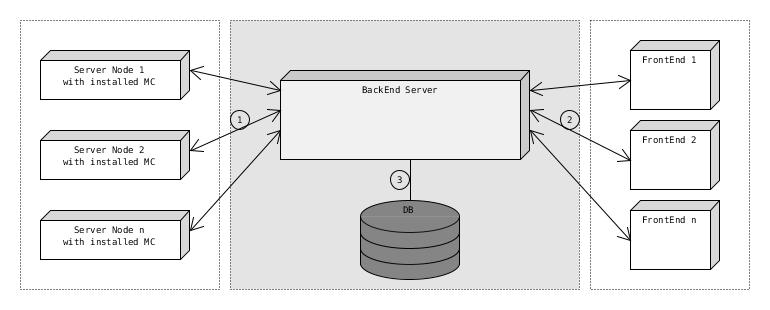
\includegraphics[width=\linewidth]{architectureFigure1.jpg}
	\caption{High level architecture of the EMS}
	\label{architectur}
\end{figure}
\subsection{Monitoring Client}
On all nodes which will be observed, MCs have to be installed. After installation, MCs automatically register themselves with the BE using a secure connection. They provide essential information about the node's state. These relevant Key Performance Indicators \textbf{(KPIs)} are periodically sent to the BE (push based).
\\ \textbf{Main functionalities:} Collecting KPIs, sending KPIs using secure channels.
\subsection{Back End Server}
The BE provides secure sockets onto which MCs are able to register themselves and send KPIs to. 
The BE processes received KPIs, forwards the edited data to the database \textbf{(DB)} and contains the business logic and controller.
\\ \textbf{Main functionalities:} Collecting KPIs, processing raw data, controlling communication, sending alerts, user authorization.

\subsection{Front End Dashboard}
The FE provides the user with a form to authenticate themselves to the BE and authorizes them to make certain changes of the BE/MC behavior. The FE is the view component of the architecture and offers representational functions of the data received from the BE. \\
\textbf{Main functionalities:} user authorization form, visualization of collected KPIs, providing an interface to alter BE settings and behavior 

\subsection{Communication Flow} 
It is important to note, that communication within the system has to be cohesive and follows a strict guideline. In the following paragraphs a brief overview of the core intent behind the communication flow is provided.
\paragraph{Between MC and BE:}The MC periodically sends KPIs to the BE. Likewise an unregistered MC can connect to the BE. From the BE settings which alter the time interval in which KPIs are sent to the MC. HTTPS is used to ensure the security of the connection. Figure \ref{architectur} \circled{1}.
\paragraph{Between BE and FE:} The FE sends authentication requests, subscription requests and customizable settings to the BE and receives authorization and data to visualize in return. To allow up-to-date visualization of the data the user requests to see, the FE is able to subscribe to WebSocket channels with the BE and the BE pushes messages about updated data whenever such is available. To allow bi-directional communication whilst upholding security of the connection WSS (WebSocketSecure, TLS based) is used. Figure \ref{architectur} \circled{2}.
\paragraph{Between BE and DB:}The BE sends edited data collected from MCs to the DB. Data is stored and can be accessed by the BE. Figure \ref{architectur} \circled{3}.
% ------------------------------------------------

\chapter{Specific Requirements} 
%#################################################

\section{User Interface}
% ------------------------------------------------
Author: Martin Binder |
Reviewer: Korbinian Simonis, Benedikt Holler
\subsubsection{Overview}
Figure \ref{navigation} shows how the website can be navigated. The login page acts as a fallback if an error occurs the user is redirected to the login and receives a notification with details on what went wrong. Only pages for which the user has permission are displayed.

\begin{figure}[h]
	\centering
	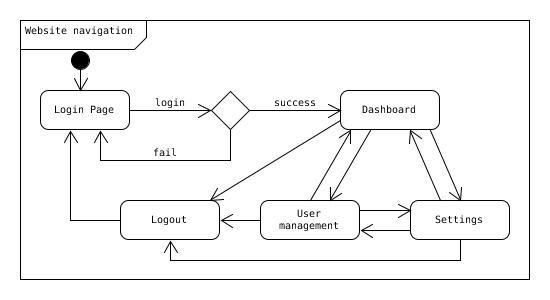
\includegraphics[width=13cm]{websiteStateChart.jpg}
	\caption{Navigation flow state chart}
	\label{navigation}
\end{figure}

\subsubsection{Login}
The first page shown upon visiting the web application is the user login on which the user can enter their credentials to access the content of the EMS.
\subsubsection{Dashboard}
\begin{figure}[h!]
	\centering
	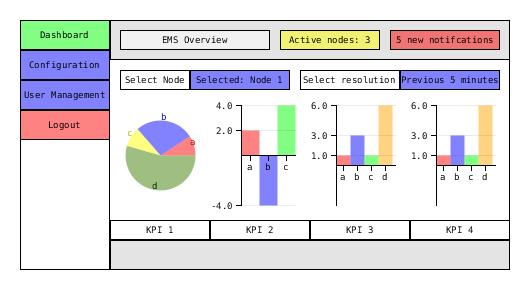
\includegraphics[width=13cm]{Dashboard.jpg}
	\caption{Rough sketch Data Representation Dashboard. Administrator View.}
	\label{dashboardConfiguration}
\end{figure}
The default page shown is the Dashboard on which data collected from the MC is graphically represented (see Figure \ref{dashboardConfiguration}). On the left side of the screen is a menu with which the user can access different functions of the application. The dashboardConfiguration provides graphical representation of a chosen KPI, which can conveniently be changed with a click on a drop down menu next to the graph to show another set of collected data from different node. Similarly, the resolution of the displayed time frame can be changed to observe the KPIs over extended time periods.
\subsubsection{Menu}
The menu on the left side shows the accessible pages for the logged in user. The currently selected page is highlighted to allow easy and comprehensible navigation. 
\subsubsection{Configuration}
If the user clicks on "Configuration" in the menu, they're redirected to the BE configuration page where they can choose which metric, condition and/or time has to be met before an alert message will be sent. Further options concerning the Backend behavior can also be accessed  from this page.
\subsubsection{User management}
If the user has adequate privileges, they can access the administration page. Here, they can change settings regarding the CRUD rights of Users or the password for the authentication process.
\subsubsection{Logout}
After a click on logout, the user session is destroyed and the User is redirected to the login screen. To access the EMS again, the User must re-authenticate. 

\section{Functions} 
Within this section, the word "shall" is used for when a function is \emph{absolutely mandatory} to be implemented and fully functional.
Likewise, the word "should" is used for when a function is \emph{desirable, but not mandatory} and will be implemented if time allows it.
% ------------------------------------------------
\subsection{Frontend (FE)}
\paragraph{F001: Secure connection to BE.} The FE shall be able to establish a secure communication channel to the BE server.
\paragraph{F002: Web-based UI.} The FE shall be usable via common browsers.
\paragraph{F003: Visualize KPIs.} The FE shall provide visualizations of the data it retrieves from the nodes.
\paragraph{F004: User login.} The FE shall prompt a user login before displaying anything else.
\paragraph{F005: User-rights based UI.} The UI shall only consist of those parts the user is entitled to access.
\paragraph{F006: User Management.} The FE shall provide masks for user management: Users shall be created, edited and deleted.
\paragraph{F007: Notifications.} Notifications shall be shown if a corresponding notification rule is fulfilled.
\paragraph{F008: User logout.} Users shall be able to sign out of the application.
\paragraph{F009: Threshold Definition.} There shall be a mask to set up and edit thresholds for every KPI.
\paragraph{F010: Alerting Rules Editor.} There shall be an editor to create, update and delete custom alerting rules.
\paragraph{F011: Data Resolution Selection.} The FE shall provide controls to select the resolution of the displayed data e.g. time, date and period.
\paragraph{F012: Reaction to Changes.} The FE shall react to changes to the currently displayed values, if such are propagated by the BE.

\subsection{Backend (BE)}
\paragraph{B001: Terminate secure connections.} The BE server shall terminate secure connections from its clients.
\paragraph{B002: User Authentication.} The BE shall only accept requests from authenticated users.
\paragraph{B003: User Management.} The BE shall take care of which users exist and what rights they have, and provide functions to create, edit and delete them.
\paragraph{B004: Mail Notifications.} The BE shall send E-mails if corresponding notification rules are fulfilled.
\paragraph{B005: Push Notifications.} The BE shall push notification to the FE if corresponding notification rules are fulfilled.
\paragraph{B006: Store Thresholds.} Thresholds for each KPI shall be configurable and be persisted.
\paragraph{B007: Custom alerting rules.} Custom alerting rules shall be available. These consist of a KPI type, a threshold, and/or a time limit, all of which shall be customizable (i.e. notification rules). If a KPI reaches the threshold or stays above a threshold for longer than the time limit, alert notifications shall be sent. These alerting rules shall be able to be created, deleted, changed and stored.
\paragraph{B008: KPI Storage.} The BE shall store all KPI values it received from the MC in a persistent, query-able way.
\paragraph{B009: MC Registration.} The BE shall accept registration requests from MCs.
\paragraph{B010: Flexible Resolution of Data.} The resolution of the requested data should be configurable with every request.
\paragraph{B011: Data Accumulation.} The BE shall provide multiple variants in which the KPI data may be requested in an accumulated way.
\paragraph{B012: Estimate Energy Consumption.} The BE shall estimate the energy consumption of  MCs if no measuring instrument is installed.
\paragraph{B013: Oscillation Handling.} The BE shall provide an option for data post-processing, so that MCs sending regularly fluctuating KPI values don't warp data aggregations and annoy the User with notifications. This option shall be configurable by the user so every user has his own settings.
\paragraph{B014: Push KPI changes.} The BE shall push changes to the KPIs that are currently displayed on the FE.
\paragraph{B015: Limited Access.} The BE shall only fulfill requests that were filed with the correct user rights.

\subsection{Monitoring Client (MC)}
\paragraph{M001: Push KPIs to BE.} The MC shall push KPIs to the BE server regularly.
\paragraph{M002: Read KPIs.} The MC shall read certain KPIs from their relevant sources.
\paragraph{M003: Configuration of MC.} The MC shall be able to retrieve relevant configuration parameters from the BE server.
\paragraph{M004: Secure connection to BE.} The MC shall establish a secure communication channel to the BE server.
\paragraph{M005: BE Registration.} The MC shall register itself with the BE server after installation.
\paragraph{M006: User Space Application.} The MC shall be fully functional with only user privileges.
\paragraph{M007: Read Energy Consumption.} The MC shall read the energy consumption from the relevant sources.

\section{Extended Criteria}
\subsection{Frontend}
\paragraph{EF001: Software Monitoring.} The FE should be able to show if a predefined software is currently running.
\paragraph{EF002: Required Software Definition.} The FE should provide a form where required software can be added and deleted.
\paragraph{EF003: Image export.} The FE should be able to create image files from the KPI visualizations and provide a function to save them.
\paragraph{EF004: Date Selection for displayed KPIs.} The FE should offer a functionality to display the collected graphical representation of a selected KPI from a certain time period picked from a calendar.
\paragraph{EF005: Data Comparison.} The FE should contain functionality to compare two data sets of either different nodes or from different time periods.

\subsection{Backend}
\paragraph{EB001: Software Monitoring.} The BE should be able to send notifications via E-mail when a predefined required software is not running.
\paragraph{EB002: Required Software Definition.} The BE should provide functions to add and delete the names of required software to monitor.

\subsection{Monitoring Client}
\paragraph{EM001: Process Monitoring.} The MC should be able to report a list of running processes to the BE.

 
\section{Constraints}
The functionality listed here is beyond the scope of the EMS and will \emph{not} be implemented.
\paragraph{C001: No Shut Down.} The EMS will not be provided with a shut down function to assure continued monitoring and prevent any alteration when the system is turned off without being recognized.
\paragraph{C002: Controlling.} The tool's main objective is the monitoring part of the nodes, controlling them is explicitly not within our scope. 
\paragraph{C003: No total insurance.} If a device within an EMS architecture does not work properly due to external reasons (e.g. outdated BE hardware), it is not a job for the EMS itself to fix these issues.
\paragraph{C004: Storing of KPI values only for a limited time.} It won't be possible to save all KPIs sent to the BE over prolonged periods of time due to disk space limitations.

\section{Performance Requirements}
% ------------------------------------------------
% Betriebs- und Qualitätsbedingungen
Author: Andreas M\"uller |
Reviewer: Benedikt Holler, Simon Sch\"onberger
\paragraph{Performance.}
For a better work flow, the website needs a short response time and (if visited frequently) page load time. \\
The EMS must not affect other applications running on the nodes (e.g. affecting runtime). \\ 
If energy demand thresholds are surpassed, users are immediately notified via E-mail.

\paragraph{Safety.}
Connection between BE and MC as well as the connection between BE and FE is secured, so no information is leaked or altered.

\paragraph{Reliability.}
Reliability has to be measured and cannot be determined at the given time.


\section{Software Quality Attributes}
Author: Andreas M\"uller |
Reviewer: Benedikt Holler, Simon Sch\"onberger 
% Betriebs- und Qualitätsbedingungen

\paragraph{Usability.}
The dashboardConfiguration needs to be able to present the different KPIs in a flexible manner, so that the end-users can easily identify the bottleneck nodes in terms of performance and energy demand. \\ Easy navigation should help users to learn and work more efficiently with our EMS. The user should be able to immediately tell what an operating element does.

\paragraph{Availability.}
Data already saved on the Backend should be available 24/7 (except if the
BE is down). If a problem occurs with the connection between BE and MC or between BE and FE, data will be sent again.

\paragraph{Security.}
Only authenticated users can access the FE and have CRUD rights, which still need to be determined.

\section{Global Scenarios and Test Cases} 
Author:  Simon Sch\"onberger |
Reviewer: Andreas M\"uller, Korbinian Simonis \\
% ------------------------------------------------

\noindent In this section we list global scenarios and test cases to ensure the functionality of the major requirements of our EMS. Unless otherwise stated, we use a standard setting explained below.
\\
\subparagraph{Standard test setting:} User is on the login page.\newline

\paragraph{GT001: Registration.} 
\subparagraph{Test case:} Administrator gives new user login information for new account.
\subparagraph{Test verification:} User enters given user name and password. User is logged in. 

\paragraph{GT002: Log in.} 
\subparagraph{Test case:} User enters user name and password.
\subparagraph{Test verification:} User can see a list of their servers.

\paragraph{GT003: Delete Users.} 
\subparagraph{Test case:} Administrator removes user account.
\subparagraph{Test verification:} User tries to login. Login fails.

\paragraph{GT005: Log out.} 
\subparagraph{Test setting:} User is logged in.
\subparagraph{Test case:} Url is cached. User clicks on “log out”.
\subparagraph{Test verification:} Call Url. User is redirected to the Login page.

\paragraph{GT006: Adding new clients.} 
\subparagraph{Test setting:} BE already connected to several MC:
\subparagraph{Test case:} Install program on new node.
\subparagraph{Test verification:} Log in. FE lists new node.

\paragraph{GT007: Change monitoring settings.} 
\subparagraph{Test setting:} User is on the setting page.
\subparagraph{Test case:} Change time interval of "KPIs sent" from five to ten seconds.
\subparagraph{Test verification:} BE only receives KPIs every ten seconds.

\paragraph{GT008: Alert-system.} 
\subparagraph{Test setting:} Add a dummy-node to the system.
\subparagraph{Test case:} Let the dummy-node have a CPU load above 80\% or let the dummy withhold information for different time periods.
\subparagraph{Test verification:} Check E-mails if the necessary E-mails are sent. Log in and see if notifications were sent.

\paragraph{GT009: Display updated data.}
\subparagraph{Test setting:} Add a dummy-node to the system. User is logged in and selected to display the energy consumption of the dummy.
\subparagraph{Test case:} Change the energy consumption of the dummy once every minute.
\subparagraph{Test verification:} Observe if and how the energy consumption changes. Compare results with dummy.
\newpage
\section{Security} 
Author: Simonis Korbinian |
Reviewer: Martin Binder, Benedikt Holler \\ \\ 
% ------------------------------------------------
In order to analyze the security requirements, we conduct a protection requirements determination according to the BSI Standard \footnote{ \url{https://www.bsi.bund.de/SharedDocs/Downloads/DE/BSI/Publikationen/ITGrundschutzstandards/BSI-Standard\_1002.pdf?\_\_blob=publicationFile\&v=1}, [Accessed: 2018-10-19]}.

\subsubsection{Determining Protection Requirements}
We used the following three basic categories of protection requirements to provide a qualitative statement. To avoid misconceptions, the categories are defined in Table \ref{schutz01}. \\
\begin{table}[h]
	\centering
	\begin{tabular}{|l|l|l|l|}
		\hline
		& \multicolumn{3}{c|}{Protection Requirements Categories}                                                                                                                                         \\ \hline
		"Normal"    & \multicolumn{3}{l|}{The impact of any loss or damage is limited and calculable.}                                                                                                                \\ \hline
		"High"      & \multicolumn{3}{l|}{The impact of any loss or damage may be considerable.}                                                                                                                      \\ \hline
		"Very High" & \multicolumn{3}{l|}{\begin{tabular}[c]{@{}l@{}}The impact of any loss or damage may be of catastrophic proportions \\ which could threaten the very survival of the organization.\end{tabular}} \\ \hline
	\end{tabular}
	\caption{Three categories of protection requirements.}
	\label{schutz01}
\end{table}

\noindent Tables \ref{schutz_02}, \ref{schutz_03} and \ref{schutz_04} are used to determine the protection requirements resulting from a potential damage scenario and its consequences. 
For the scenarios, we specially considered the loss of confidentiality, integrity, or availability for a particular business process or application, including its data. 
The tables are adapted to our specific situation.
\begin{table}[h]
	\centering
	\scriptsize
	\begin{tabular}{|l|l|}
		\hline
		\multicolumn{2}{|c|}{Protection requirements category "Normal"}                                                                                                                                                                                                                                        \\ \hline
		1. Violations of laws, regulations, or contracts                                                          & \begin{tabular}[c]{@{}l@{}}- Violations of regulations and laws with minor \\ consequences \\- Minor breaches of contract which result in \\ at most minor contractual penalties\end{tabular} \\ \hline
		\begin{tabular}[c]{@{}l@{}}2. Impairment of the right to \\ informational self-determination\end{tabular} & \begin{tabular}[c]{@{}l@{}}- This deals with personal data whose processing could \\ adversely affect the social standing or financial well-\\ being of those concerned.\end{tabular}        \\ \hline
		3. Physical injury                                                                                        &- Does not appear possible.                                                                                                                                                                  \\ \hline
		4. Impaired ability to perform tasks                                                                      & \begin{tabular}[c]{@{}l@{}}- Impairment was assessed to be tolerable by those \\ concerned. \\- The maximum acceptable downtime is greater than 24 \\ hours.\end{tabular}                     \\ \hline
		\begin{tabular}[c]{@{}l@{}}5. Negative internal or external \\ effects\end{tabular}                       & \begin{tabular}[c]{@{}l@{}}- Only minimal impairment or only internal impairment of \\ the reputation / trustworthiness of the organization is \\ expected.\end{tabular}                     \\ \hline
		6. Financial consequences                                                                                 &- The financial loss is smaller than 10 Euro                                                                                                                                   \\ \hline
	\end{tabular}
	\caption{Damage scenarios for the category "Normal"}
	\label{schutz_02}
\end{table}

\begin{table}[h]
	\centering
	\scriptsize
	\begin{tabular}{|l|l|}
		\hline
		\multicolumn{2}{|c|}{Protection requirements category "High"}                                                                                                                                                                                                                                                                                          \\ \hline
		1. Violations of laws, regulations, or contracts                                                          & \begin{tabular}[c]{@{}l@{}}- Violations of regulations and laws with substantial \\ consequences \\- Major breaches of contract with high contractual \\ penalties\end{tabular}                                                               \\ \hline
		\begin{tabular}[c]{@{}l@{}}2. Impairment of the right of \\ informational self-determination\end{tabular} & \begin{tabular}[c]{@{}l@{}}- This aspect deals with personal data whose processing \\ could have a seriously adverse affect on the social \\ standing or financial well-being of those concerned.\end{tabular}                               \\ \hline
		3. Physical injury                                                                                        & \begin{tabular}[c]{@{}l@{}}- Does not appear possible. \end{tabular}                                                                                                                                \\ \hline
		4. Impaired ability to perform tasks                                                                      & \begin{tabular}[c]{@{}l@{}}- Impairment of the ability to perform the tasks at hand \\ was assessed as intolerable by some of the individuals \\ concerned. \\- The maximum acceptable downtime is between one and \\ 24 hours.\end{tabular} \\ \hline
		\begin{tabular}[c]{@{}l@{}}5. Negative internal or external \\ effects\end{tabular}                       & \begin{tabular}[c]{@{}l@{}}- Considerable impairment of the \\ reputation/trustworthiness can be expected.\end{tabular}                                                                                                                      \\ \hline
		6. Financial consequences                                                                                 & \begin{tabular}[c]{@{}l@{}}- The financial loss is between 10 and 100 Euro\end{tabular}                                                                                                    \\ \hline
	\end{tabular}
	\caption{Damage scenarios for the category "High"}
	\label{schutz_03}
\end{table}

\begin{table}[h]
	\centering
	\scriptsize
	\begin{tabular}{|l|l|}
		\hline
		\multicolumn{2}{|c|}{Protection requirements category "Very High"}                                                                                                                                                                                                                                                                                      \\ \hline
		1. Violations of laws, regulations, or contracts                                                          & \begin{tabular}[c]{@{}l@{}}- Fundamental violations of regulations and laws\\ - Breaches of contract with ruinous damage liabilities\end{tabular}                                                                                           \\ \hline
		\begin{tabular}[c]{@{}l@{}}2. Impairment of the right of \\ informational self-determination\end{tabular} & \begin{tabular}[c]{@{}l@{}}- This aspect deals with personal data whose processing \\ could result in the injury or death of the persons \\ concerned or that could endanger the personal freedom \\ of the persons concerned.\end{tabular} \\ \hline
		3. Physical injury                                                                                        & \begin{tabular}[c]{@{}l@{}}- Physical injury to an individual cannot be absolutely 
			ruled out.  \end{tabular}                                                                                                              \\ \hline
		4. Impaired ability to perform tasks                                                                      & \begin{tabular}[c]{@{}l@{}}- Impairment of the ability to perform tasks was assessed \\ as intolerable by all individuals concerned.\\ - The maximum acceptable downtime is less than one \\ hour.\end{tabular}                         \\ \hline
		\begin{tabular}[c]{@{}l@{}}5. Negative internal or external \\ effects\end{tabular}                       & \begin{tabular}[c]{@{}l@{}}- A nation-wide or state-wide loss of \\ reputation/trustworthiness is conceivable, possibly\\ even endangering the existence of the organization.\end{tabular}                                                  \\ \hline
		6. Financial consequences                                                                                 & \begin{tabular}[c]{@{}l@{}}- The financial loss is more than 100 Euro \end{tabular}                                                                                                                                \\ \hline
	\end{tabular}
	\caption{Damage scenarios for the category "Very High"}
	\label{schutz_04}
\end{table}

\noindent Table \ref{schutz_app} shows the main applications, their protection requirements, and the reasons for selecting the given protection requirements.

\begin{table}[h]
	\scriptsize
	\centering
	\begin{tabular}{|
			>{\columncolor[HTML]{FFCCC9}}l |c|c|c|c|}
		\hline
		\multicolumn{2}{|c|}{\cellcolor[HTML]{FFCCC9}Application} & \multicolumn{3}{c|}{\cellcolor[HTML]{FFCCC9}Protection Requirements}                                                                                                                                                                             \\ \hline
		No.            & \cellcolor[HTML]{FFCCC9}Label            & \cellcolor[HTML]{FFCCC9}Basic Value & \cellcolor[HTML]{FFCCC9}Protection Requirements & \cellcolor[HTML]{FFCCC9}Reasons                                                                                                                          \\ \hline
		A1             & Monitoring Dashboard                     & Confidentiality                     & Normal                                          & \begin{tabular}[c]{@{}c@{}}No confidential data is generated or stored.\\ The protection requirement is normal.\end{tabular}                             \\ \hline
		&                                          & Integrity                           & High                                            & \begin{tabular}[c]{@{}c@{}}Untampered view of the KPIs is essential for\\ the user.\end{tabular}                                                         \\ \hline
		&                                          & Availability                        & High                                            & \begin{tabular}[c]{@{}c@{}}All users are affected by downtimes. \\ Failure of this system is therefore acceptable \\ at best for 24 hours.\end{tabular} \\ \hline
		A2             & Monitoring Client                        & Confidentiality                      & Normal                                          & \begin{tabular}[c]{@{}c@{}}No confidential data is generated or stored.\\ The protection requirement is normal.\end{tabular}                             \\ \hline
		&                                          & Integrity                           & High                                            & \begin{tabular}[c]{@{}c@{}}Providing untampered data is essential for\\ a monitoring software.\end{tabular}                                              \\ \hline
		&                                          & Availability                        & Normal                                          & \begin{tabular}[c]{@{}c@{}}Affects only single nodes.\\ Downtimes can be handled via manual surveillance.\end{tabular}                                 \\ \hline
	\end{tabular}
	\caption{Protection requirements for our applications}
	\label{schutz_app}
\end{table}

\noindent The protection requirements of the applications are included in the determination of protection requirements for the respective IT systems. (Table \ref{schutz_sys} ). We used the maximum principle, since we follow the BSI Standard, which means, that we have to consider the total potential damage to relevant applications on the respective IT system. 

\begin{table}[h]
	\centering
	\scriptsize
	\begin{tabular}{|
			>{\columncolor[HTML]{FFCCC9}}l |c|c|l|l|}
		\hline
		\multicolumn{2}{|l|}{\cellcolor[HTML]{FFCCC9}IT System} & \multicolumn{3}{c|}{\cellcolor[HTML]{FFCCC9}Protection Requirements}                                                    \\ \hline
		No.            & \cellcolor[HTML]{FFCCC9}Label           & \cellcolor[HTML]{FFCCC9}Basic Value & \cellcolor[HTML]{FFCCC9}Protection Requirements & \cellcolor[HTML]{FFCCC9}Reasons \\ \hline
		S1             & Backend server                    & Confidentiality                      & Normal                                            & Maximum principle according to application A1      \\ \hline
		&                                          & Integrity                           & High                                               & Maximum principle according to application A1        \\ \hline
		&                                          & Availability                        &  High                                               & Maximum principle according to application A1          \\ \hline
		C2             & Client Servers                        & Confidentiality                      &   Normal                                              &   Maximum principle according to application A2             \\ \hline
		&                                          & Integrity                           & High                                      & Maximum principle according to application A2             \\ \hline
		&                                          & Availability                        &    Normal                                             & Maximum principle according to application A2              \\ \hline
	\end{tabular}
	\caption{Protection requirements for our IT system}
	\label{schutz_sys}
\end{table}

\noindent Once the determination of the protection requirements for the applications and IT systems being examined has been completed, the protection requirements for the networking structure must be determined. Points \circled{1} and \circled{2} in Figure \ref{architectur} show our connections. \circled{1} is the connection from the MC to the BE and \circled{2} is the connection from the BE to the FE. Even if the connections in our particular case take place within the Intranet, our system shall also provide the necessary security for connections via the Internet, as 'geographically dispersed' does not necessarily refer to an Intranet use only. For this reason, we consider in Table \ref{schutz_con} both connections are to the outside world, which means that they lead into or through uncontrolled area, such as the Internet.

% Please add the following required packages to your document preamble:
% \usepackage[table,xcdraw]{xcolor}
% If you use beamer only pass "xcolor=table" option, i.e. \documentclass[xcolor=table]{beamer}
\begin{table}[h!]
	\centering
	\scriptsize
	\begin{tabular}{|
			>{\columncolor[HTML]{FFCCC9}}c |c|c|c|c|c|}
		\hline
		& \multicolumn{5}{c|}{\cellcolor[HTML]{FFCCC9}Critical because}                                                                                                                                                                                                                                                                                         \\ \hline
		Connection                             & \begin{tabular}[c]{@{}c@{}}K1\\ Outside\\ connection\end{tabular} & \begin{tabular}[c]{@{}c@{}}K2\\ Highly\\ Confidential\end{tabular} & \begin{tabular}[c]{@{}c@{}}K3\\ High\\ Integrity\end{tabular} & \begin{tabular}[c]{@{}c@{}}K4\\ High\\ Availability\end{tabular} & \begin{tabular}[c]{@{}c@{}}K5\\ Transmission\\ not permitted\end{tabular} \\ \hline
		MC - BE (\circled{1}) & X                                                                 &                                                                    &                                                               &                                                                  &                                                                           \\ \hline
		BE - FE (\circled{2}) & X                                                                 &                                                                    &                                                               &                                                                  &                                                                           \\ \hline
	\end{tabular}
	\label{schutz_con}
\end{table}


\chapter{DevOps and Tooling} 
Author: Simon Sch\"onberger |
Reviewer: Andreas M\"uller, Martin Binder
\section{Collaboration} 
To successfully develop software as a team, it is fundamental to agree on a collaboration
platform that will be consequently used to communicate any task, effort, question
made in order to deliver the project's assets.
As such platform we chose \emph{YouTrack}, an issue tracker and agile collaboration tool made
by JetBrains, which will integrate well with our IDE (see \ref{devops-ide}).
YouTrack provides us with the following capabilities:
\begin{itemize}
  \item Issue Tracking.
  \item An agile board to track down our efforts including agile progress tracking like
    Burn-down-charts.
  \item Maintenance of a product backlog.
\end{itemize}
When a new sprint is planned, all team members will record tasks and user stories in
YouTrack. Additionally time estimation, prioritization and allocation to certain team members 
will be conducted in accordance with the responsible Product Owner.\\
The team will use 3 stages to track the progress in each sprint. \\
\textbf{1. Draft phase:} This phase will start at Wednesday with the start of the sprint. Team members start working on their task and create a rough draft which can be presented to the customer on the following Wednesday to show the direction in which the team is heading, allow the team to collect valuable feedback and recognize issues early on. The time units estimated for each task will be equally split between the three phases.  \\
\textbf{2. Refinement phase:} Phase one and two will have a smooth transition, as soon as a team member finishes their allocated drafts they can start working on the version which will be presented to the customer. \\  
\textbf{3. Verify phase:} After the refinement is done the PO will allocate the result to two other team members to check on the work and give feedback to the author who will then proceed to finish the task with regard of the feedback.
Every comment, question or feedback will be recorded with YouTrack to enable swift processing of each task and allow the PO/SCM to keep a clear overview of the progress.\\
This method might change with the requirements of certain sprint phases.\\
\fbox{\parbox{0.93\linewidth}{
    Our YouTrack instance is available at \href{https://enpr01.fim.uni-passau.de/youtrack/}{https://enpr01.fim.uni-passau.de/youtrack/}.
}}

\section{VCS}
Version Control Systems provide an established and easy way of concurrently working on
large sets of data like our software project. We will use \emph{Git} as a distributed Version
Control System. Git provides us with a central repository that will contain the current
state of our work and is readable and writable by all team members. As a Frontend for
easily browsing the repository we use Gitea. \\

\fbox{\parbox{0.93\linewidth}{
    Our Git instance is reachable via HTTPS and SSH at git@enpr01.fim.uni-passau.de. The Gitea Frontend is available at \href{https://enpr01.fim.uni-passau.de/git/}{https://enpr01.fim.uni-passau.de/git/}.
}}

\section{IDEs}
\label{devops-ide}
The team agreed on using \emph{IntelliJ IDEA} by JetBrains for working on the project, as it
provides great integration with YouTrack and Git and allows a smooth collaboration and helps coordinate the combined efforts of the team through many helpful
features regarding code-completion, refactoring or build-system-integration. \\
For any other purpose than editing code, the use of the greatest of all text editors, \emph{vim} is strongly recommended.

\section{Platform}
Development will take place on \emph{Linux}. Even though it is crucial to have at least
one MS Windows machine available to allow compatibility testing of our software.

\end{document}
